\documentclass[12pt]{article}
\usepackage{enumerate}
\usepackage{notes}
\usepackage{oxford}

\begin{document}
\title{Oxford A0 - Linear Algebra \footnotetext{\url{https://courses.maths.ox.ac.uk/node/5353}}}
\author{Dan Davison}
\maketitle

\section*{Sheet 1}

\subsection*{} % 1
\begin{mdframed}
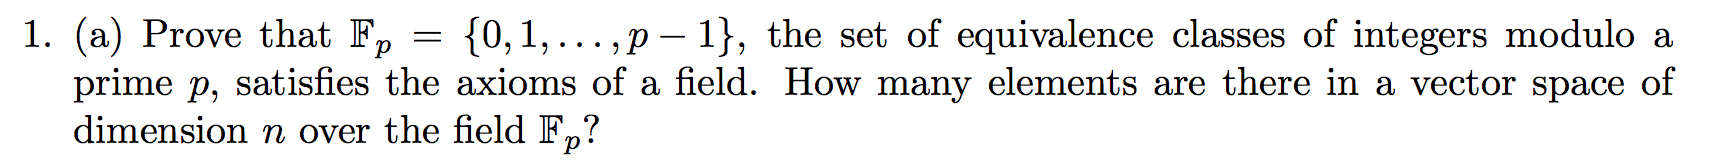
\includegraphics[width=450pt]{img/linear-algebra-a0-1-1-a.png}\\
\end{mdframed}

Let\footnote{Unlike the question, I am trying to use notation that
  distinguishes between integers and their equivalence classes.}
$a, b, c \in \Z$ with $0 \leq a < p, ~~ 0 \leq b < p, ~~ 0 \leq c < p$.

Let $\bar a, \bar b, \bar c \in \F$ be equivalence classes of integers modulo $p$.

The field axioms are listed below, together with proof that they hold for $\F_p$.
\begin{enumerate}
\item \textbf{$\F_p$ is an abelian group under addition}\\
  Define $\bar a + \bar b := \bar{a + b}$, then:
  \begin{enumerate}
  \item \textit{Existence of identity}: $\bar 0$ is the identity since
    $\bar a + \bar 0 = \bar{a + 0} = \bar{a}$ for all $\bar a \in \F_p$.
  \item \textit{Existence of inverses}: $(\bar a)^\1 = \bar{-a}$ since
    $\bar a + \bar{-a} = \bar{a + -a} = \bar{0}$ for all $a \in \F_p$.
  \item \textit{Commutativity}:
    $\bar a + \bar b = \bar{a + b} = \bar{b} + \bar{a}$ for all $a, b \in \F_p$.
  \item \textit{Associativity}:
    $\bar a + (\bar b + \bar c) = \bar a + \bar {b + c} = \bar{a + b + c} =
    \bar{a + b} + \bar{c} = (\bar a + \bar b) + \bar{c}$.
  \end{enumerate}
\item \textbf{$\F_p\setminus\{\bar 0\}$ is an abelian group under multiplication}\\
  Define $\bar a ~ \bar b := \bar{ab}$, then:
  \begin{enumerate}
  \item \textit{Existence of identity}: $\bar 1$ is the identity since
    $\bar a \bar 1 = \bar{a\cdot 1} = \bar{a}$ for all $\bar a \in \F_p$.
    \newpage
  \item \textit{Existence of inverses for everything except additive identity}:\\\\
    The claim is that for all $\bar a \in \F_p \setminus \{\bar 0\}$ there
    exists $\bar b \in \F_p$ such that $\bar a ~ \bar b = \bar 1$.

    Fix an arbitrary $a \in \{1, \ldots, p-1\}$.

    The claim is equivalent to the following: there exists
    $b \in \{0, 1, \ldots, p\}$ such that for all $i, j \in \Z$ there exists
    $k \in \Z$ such that $(ip + a)(jp + b) = kp + 1$.

    But note that $(ip + a)(jp + b) = p(ijp + aj + bi) + ab$ and therefore
    \begin{align*}
      &(ip + a)(jp + b) = kp + 1\\
      \iff &ab = p(k - ijp - aj - bi) + 1.
    \end{align*}
    Since $k$ can be chosen freely, the condition is simply that for all
    $i, j \in \Z$ there exists $k \in \Z$ such that $ab = kp + 1$.

    Note\footnote{I eventually allowed myself to google for a hint here which
      brought up people pointing to Bezout's identity.} that $a$ and $p$ are
    coprime (gcd is 1). By Bezout's identity, there exists $b, -k \in \Z$
    such that
    \begin{align*}
      ba + (-k)p = 1 \iff ab = kp + 1. \qed
    \end{align*}


  \item \textit{Commutativity}:
    $\bar a ~ \bar b = \bar{ab} = \bar{b} ~ \bar{a}$ for all $a, b \in \F_p$.
  \item \textit{Associativity}:
    $\bar a (\bar b \bar c) = \bar a + \bar {bc} = \bar{abc} =
    \bar{ab}~\bar{c} = (\bar a ~ \bar b) \bar{c}$.
  \end{enumerate}
\item \textbf{Distributive axiom}
  \begin{enumerate}
  \item \textit{Multiplication distributes over addition}: $\bar a (\bar b + \bar c) = \bar a (\bar{b + c}) = \bar{a(b+c)} = \bar{ab +
    ac} = \bar{ab} + \bar{ac} = \bar{a}~\bar{b} + \bar{a}~\bar{c}$
  \end{enumerate}
\end{enumerate}

There are $p^n$ elements in a vector space of dimension $n$ over the field $\F_p$.
\newpage
\begin{mdframed}
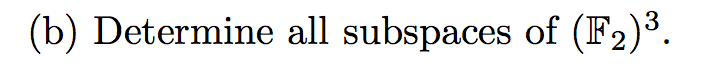
\includegraphics[width=200pt]{img/linear-algebra-a0-1-1-b.png}
\end{mdframed}

\textit{Remark}: This is like the 8 vectors that form the unit cube in
$\R^3$, except that when extended beyond the cube by vector addition or
scalar multiplication they ``wrap around''.

Note that
\begin{align*}
  (\F_2)^3 = \{&\bar 0, \bar 1\}^3\\
           = \{&(\bar 0, \bar 0, \bar 0),\\
               &(\bar 0, \bar 0, \bar 1),\\
               &(\bar 0, \bar 1, \bar 0),\\
               &(\bar 0, \bar 1, \bar 1),\\
               &(\bar 1, \bar 0, \bar 0),\\
               &(\bar 1, \bar 0, \bar 1),\\
               &(\bar 1, \bar 1, \bar 0),\\
               &(\bar 1, \bar 1, \bar 1)\}.
\end{align*}
The set of subspaces of $(\F_2)^3$ is
\begin{align*}
  &\{\{(\bar 0, \bar 0, \bar 0)\}\} ~~~~~~~~~~~~~~~~~~~~~ \cup\\
  &\{\{(\bar 0, \bar 0, \bar 0), x\} ~|~ x \in (\F_2)^3\} ~~~ \cup\\
  &\{\{(\bar 0, a, b) ~|~ a, b \in \F_2\}\}  ~~~~~~~ \cup\\
  &\{\{(a, \bar 0, b) ~|~ a, b \in \F_2\}\}  ~~~~~~~ \cup\\
  &\{\{(a, b, \bar 0) ~|~ a, b \in \F_2\}\}  ~~~~~~~ \cup\\
  &\{(\F_2)^3\}.
\end{align*}


\newpage
\subsection*{} % 2
\begin{mdframed}

\includegraphics[width=450pt]{img/linear-algebra-a0-1-2.png}\\
\end{mdframed}
We need to:
\begin{enumerate}
\item \textbf{\textit{Exhibit a proper subspace $S[x] \subset \R[x]$ and a bijection $f:\R[x] \to S[x]$}}\\\\
  Let $a_i \in \R$ for $i = 0, 1, 2, \ldots$ so that
  $\R[x] = \{a_0 + a_1x^1 + a_2x^2 + \ldots\}$.

  Define $S[x] = \{0 + a_1x^1 + a_2x^2 + a_3x^3 + \ldots\}$, i.e. the restriction
  of $\R[x]$ to those polynomials that have constant term zero.

  $S[x]$ is a proper subspace of $\R[x]$ since it contains the zero polynomial,
  and is closed under addition and scalar multiplication.

  Define $f: \R[x] \to S[x]$ where
  $f(a_0 + a_1x^1 + a_2x^2 + \ldots) = 0 + a_0x^1 + a_1x^2 + a_2x^3 + \ldots$.

  $f$ is clearly injective, since if $f(r(x)) = f(r'(x))$ then their
  coefficients $a_0, a_1, \ldots$ are the same and hence $r(x) = r'(x)$.

  Also, $f$ is clearly surjective since if
  $s(x) = a_1x^1 + a_2x^2 + a_3x^3 + \ldots$ then
  $s(x) = f(a_1 + a_2x^1 + a_3x^2 + \ldots)$.

\item \textbf{\textit{Prove that $f$ preserves addition}}\\\\
  Let $a_i,b_i \in \R$ for $i = 0, 1, 2, \ldots$

  Let $r(x) = a_0 + a_1x^1 + a_2x^2 + \ldots$ and $r'(x) = b_0 + b_1x^1 + b_2x^2 + \ldots$.

  Then
  \begin{align*}
    f\Big(r(x) + r'(x)\Big)
    &= f\Big((a_0 + b_0) + (a_1 + b_1)x^1 + (a_2 + b_2)x^2 + \ldots\Big)\\
    &= 0 + (a_0 + b_0)x^1 + (a_1 + b_1)x^2 + (a_2 + b_2)x^3 + \ldots\\
    &= \Big(0 + a_0x^1 + a_1x^2 + a_2x^3 + \ldots \Big) \\
    &+ \Big(0 + b_0x^1 + b_1x^2 + b_2x^3 + \ldots \Big) \\
    &= f\Big(r(x)\Big) + f\Big(r'(x)\Big).
  \end{align*}

  \begin{align*}
  \end{align*}

\item \textbf{\textit{Prove that $f$ preserves scalar multiplication}}
  \begin{align*}
    f\Big(\lambda r(x)\Big)
    &= f\Big(\lambda a_0 + \lambda a_1x^1 + \lambda a_2x^2 + \ldots \Big) \\
    &= 0 + \lambda a_0x^1 + \lambda a_1x^2 + \lambda a_2x^3 + \ldots \\
    &= \lambda(0 + a_0x^1 + a_1x^2 + a_2x^3 + \ldots) \\
    &= \lambda f\Big(r(x)\Big)
  \end{align*}


\end{enumerate}

\newpage
\subsection*{} % 3
\begin{mdframed}
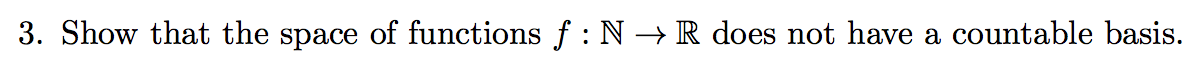
\includegraphics[width=400pt]{img/linear-algebra-a0-1-3.png}\\

Note:
\begin{enumerate}
\item The space of functions $f:\N \to \R$ is the space of real-valued
infinite sequences.
\item A basis is countable iff a bijection exists between the basis and $\N$.
\end{enumerate}

Let $x_i \in \R$ for $i \in \N$ and define the following:
\begin{itemize}
\item $F_n := \{(x_1, x_2, \ldots, x_n) ~|~ x_1, x_2, \ldots, x_n \in \R\}$ is
  the space of functions\\$f:\{1,2, \ldots, n\} \to \R$;
\item $F_\infty := \{(x_1, x_2, \ldots) ~|~ x_1, x_2, \ldots \in \R\}$ is the
  space of functions $f:\N \to \R$.
\end{itemize}

Note that $F_1 = \{x_1 ~|~ x_1 \in \R\} = \R$. Therefore every basis for $F_1$ has cardinality
1 (every basis is a set containing a single non-zero real number).

Similarly, $F_2 = \R^2$, and every basis of $F_2$ has cardinality 2.

\red{Doesn't this suggest, contra the question, that every basis of $F_\infty$ is countable?}

\end{mdframed}

\subsection*{} % 4
\begin{mdframed}
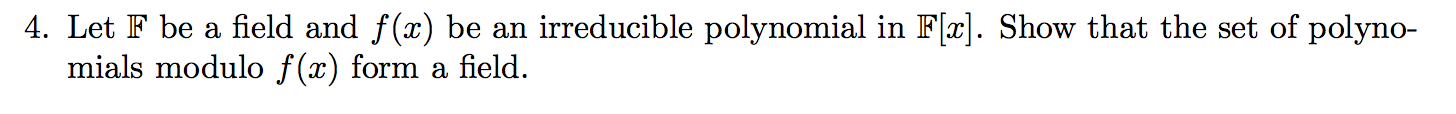
\includegraphics[width=400pt]{img/linear-algebra-a0-1-4.png}\\
\end{mdframed}
We need to show
\begin{enumerate}
\item \textbf{Addition yields an abelian group}
  \begin{enumerate}
  \item The additive identity is $\bar 0$, i.e. the equivalence class of the zero polynomial.
  \item For an arbitrary element $\bar{g(x)}$ its additive inverse is $\bar{-g(x)}$
  \item Addition is commutative and associative
  \end{enumerate}
\item \textbf{Multiplication yields an abelian group}
\item \textbf{Multiplication distributes over addition}
\end{enumerate}

\subsection*{} % 5
\begin{mdframed}
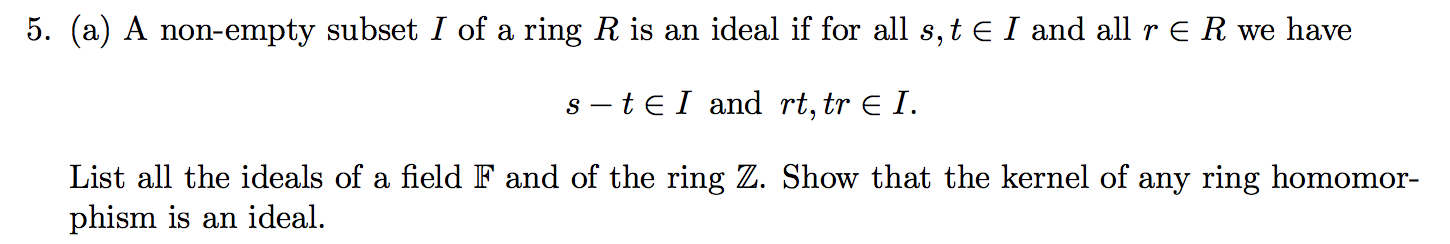
\includegraphics[width=400pt]{img/linear-algebra-a0-1-5-a.png}\\
\end{mdframed}
\begin{mdframed}
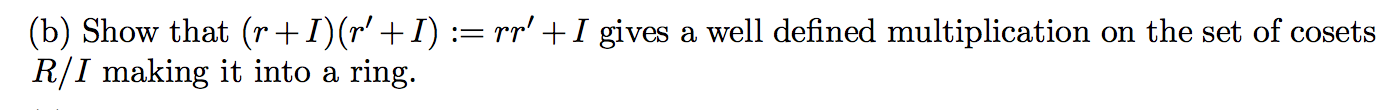
\includegraphics[width=400pt]{img/linear-algebra-a0-1-5-b.png}\\
\end{mdframed}
\begin{mdframed}

\includegraphics[width=280pt]{img/linear-algebra-a0-1-5-c.png}\\
\end{mdframed}

\subsection*{} % 6
\begin{mdframed}
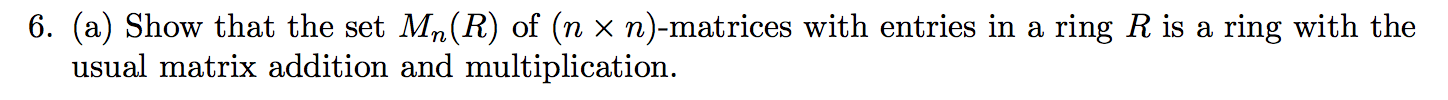
\includegraphics[width=400pt]{img/linear-algebra-a0-1-6-a.png}\\
\end{mdframed}
\begin{mdframed}
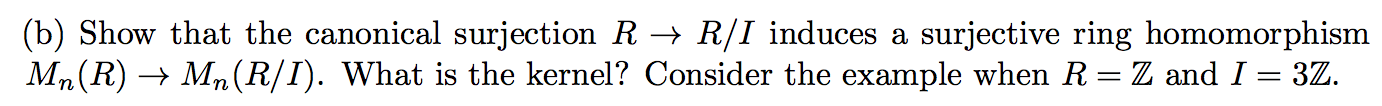
\includegraphics[width=400pt]{img/linear-algebra-a0-1-6-b.png}\\
\end{mdframed}
\begin{mdframed}

\includegraphics[width=350pt]{img/linear-algebra-a0-1-6-c.png}\\
\end{mdframed}

\subsection*{} % 7
\begin{mdframed}
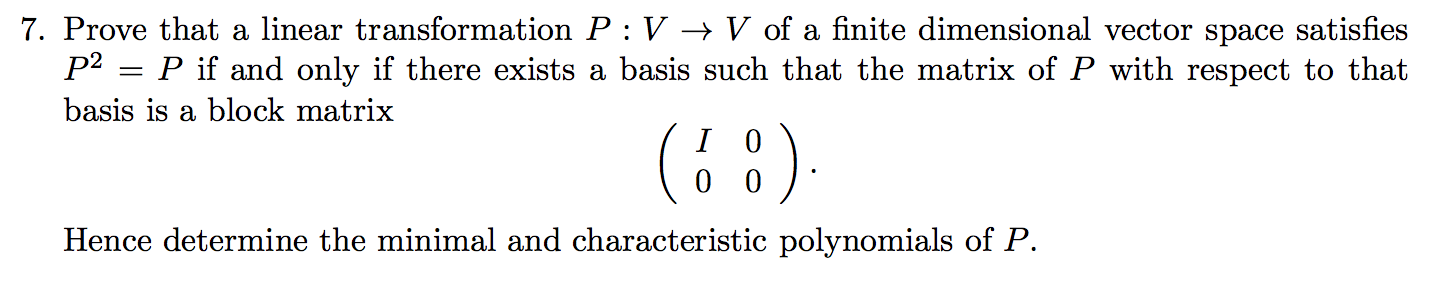
\includegraphics[width=400pt]{img/linear-algebra-a0-1-7.png}\\
\end{mdframed}

\subsection*{} % 8
\begin{mdframed}
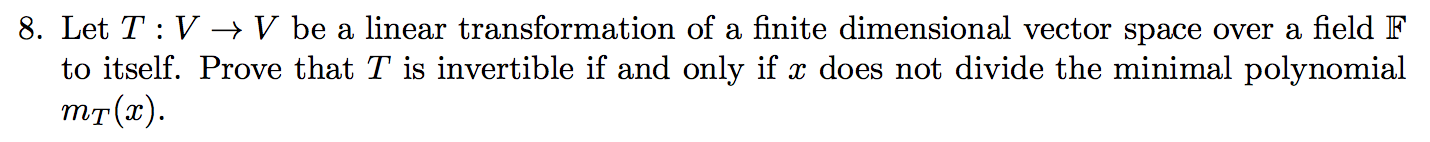
\includegraphics[width=400pt]{img/linear-algebra-a0-1-8.png}\\
\end{mdframed}

\subsection*{} % 9
\begin{mdframed}
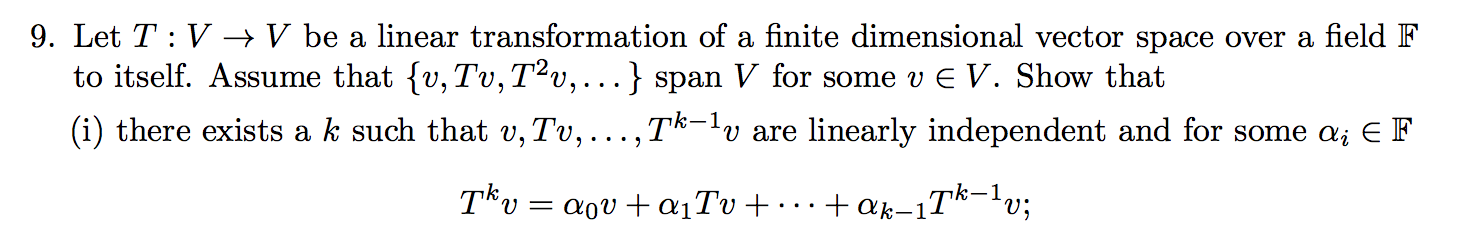
\includegraphics[width=400pt]{img/linear-algebra-a0-1-9-a.png}\\
\end{mdframed}
\begin{mdframed}
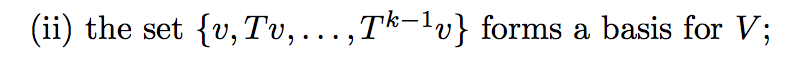
\includegraphics[width=280pt]{img/linear-algebra-a0-1-9-b.png}\\
\end{mdframed}
\begin{mdframed}
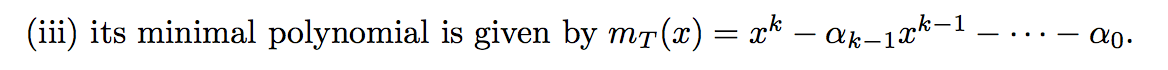
\includegraphics[width=400pt]{img/linear-algebra-a0-1-9-c.png}\\
\end{mdframed}
\begin{mdframed}

\includegraphics[width=270pt]{img/linear-algebra-a0-1-9-d.png}\\
\end{mdframed}

\end{document}
